\documentclass{article} % For LaTeX2e
\usepackage{iclr2019_conference,times}
\usepackage{times}
\usepackage{helvet}
\usepackage{courier}
\usepackage{graphicx}
\usepackage{hyperref}
\usepackage{url}
\usepackage{graphicx}
\usepackage{amsmath}
\usepackage{amsfonts}
\usepackage{todonotes}
\usepackage{epstopdf}
\usepackage{color}
\usepackage{verbatim}
\usepackage{pdfpages}
\usepackage{ amssymb }
\usepackage{caption}
\usepackage{subcaption}
\usepackage{float}
 \usepackage{booktabs}
 \usepackage{colortbl}
 \usepackage{tabularx}

% \renewcommand{\arraystretch}{1.2}
%\frenchspacing

\title{Classification of Cheatgrass Invasion using Biophysical and Remote Sensing Data}

\author{Aaron Tuor  \& Kyle Larson \\
Pacific Northwest National Laboratory\\
\texttt{\{aaron.tuor, kyle.larson\}@pnnl.gov}}

\newcommand{\fix}{\marginpar{FIX}}
\newcommand{\new}{\marginpar{NEW}}

\iclrfinalcopy % Uncomment for camera-ready version, but NOT for submission.
\begin{document}
    \maketitle

\begin{abstract} 
In this study we explore machine learning approaches which incorporate geophysical data and readings from multiple remote sensing platforms  for predictive mapping of vegetation over very large, ecologically diverse regions. 
We focus specifically on mapping an invasive exotic annual grass, cheatgrass ({\em Bromus tectorum}), that has become a major land management issue in the Western United States. We explore the advantages of integrating imagery from both the LandSat7 and MODIS platforms which have complementary spectral bandwidth, spatial resolution, and temporal frequency. Our experiments demonstrate that machine learning methods integrating biophysical variables and imagery from multiple platforms can be beneficial to the predictive mapping of invasive vegetation. Our best performing model is used to create a map of coverage predictions to aid in land management over 288 million acres of the Western United States. 
 \end{abstract}

%============================================================================================
%============================================================================================
%Section: Introduction================================================
%=============================================================================================
%============================================================================================
 \section{Introduction}
Accurate and up to date maps of vegetation coverage are critical assets for land management agencies tasked with mitigating damage wrought by invasive species. 
Current methods for mapping invasive annual grasses from satellite and aerial imagery usually involve choosing one platform. However multiple platforms may potentially be useful, e.g.,  using finer spatial resolution imagery typically improves prediction, but platforms with more frequent temporal resolution are also important for detecting invasive species which maintain growth cycles distinct from native vegetation. In this work we demonstrate the effectiveness of machine learning models which integrate biophysical data and multiple satellite platfroms.

Introduced in the late 19th-century, cheatgrass is now found in every state in the contiguous U.S. Most prevalent in western states, it has become a dominant component in many shrubland and grassland ecosystems. 
Cheatgrass invasion poses a variety of threats to ecosystem function, rangeland health, and human safety. A central thread to many of these threats is the increase in fine fuels, which can lead to increased fire frequency and irreversible loss of native vegetation and wildlife habitat. Following a fire, cheatgrass is able to more effectively compete with native vegetation, giving rise to a positive feedback cycle of further invasion and fire.\texttt{ [Refs: Mack 1981; Pellant 1996; Bradley \& Mustard 2005; USDA Plant Database]}

While cheatgrass is considered ubiquitous throughout much of the western U.S., detailed spatial information about its presence and abundance are still lacking across this extent. Our study area encompasses the U.S. portion of the sage-grouse range, which is approximately 288 million acres.
Figure \ref{fig:studyarea} shows the region considered and location of field samples we use as ground truth for training predictive models.

\begin{figure}
\centering
\begin{minipage}{.5\textwidth}
  \centering
  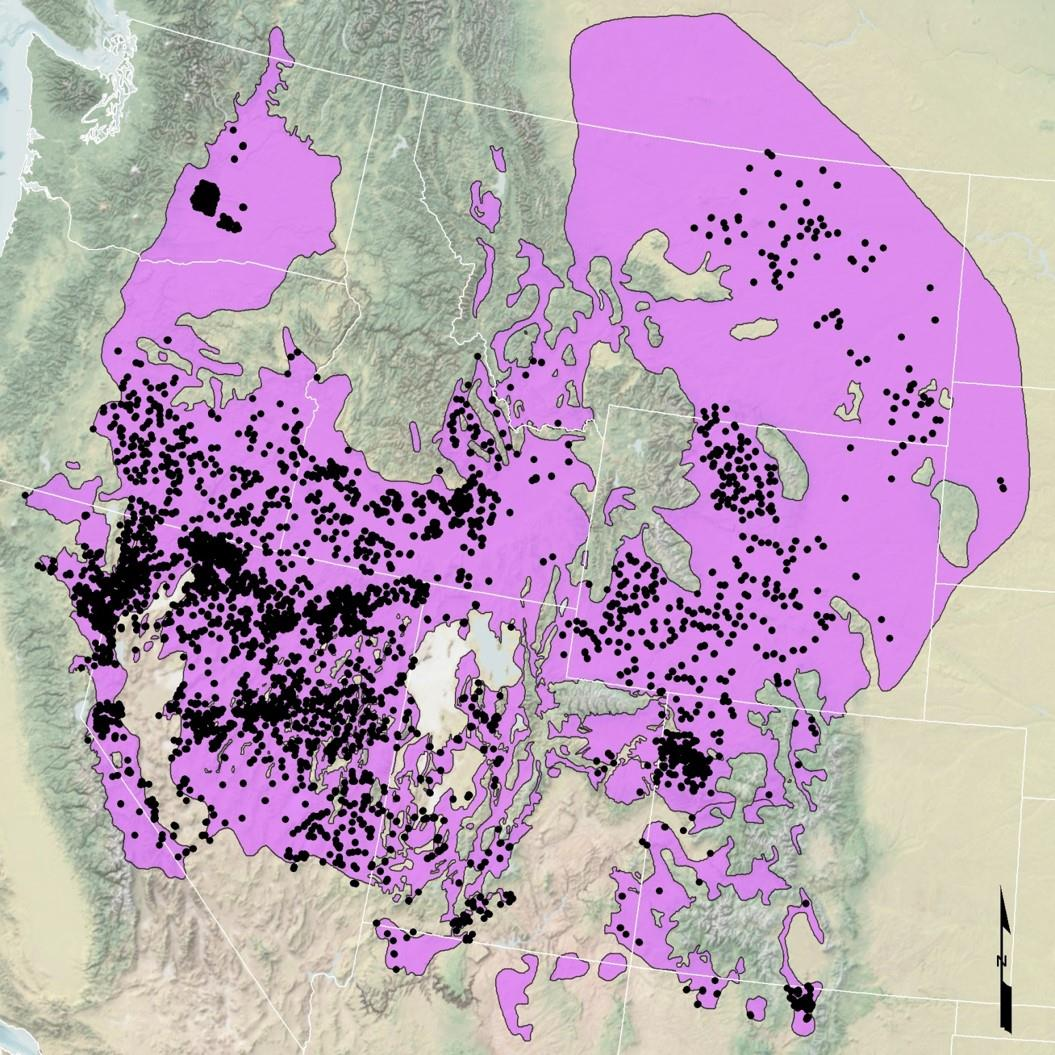
\includegraphics[width=\textwidth]{pics/studyarea.png}
 \caption{Study Region}\label{fig:studyarea}
\end{minipage}%
\begin{minipage}{.5\textwidth}
  \centering
  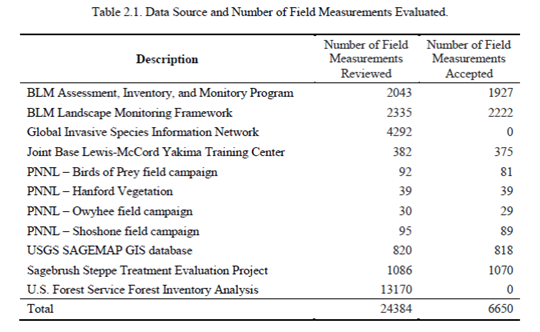
\includegraphics[width=\textwidth]{pics/fielddata.png}
\caption{Field Data}\label{fig:field}
\end{minipage}
\end{figure}
%============================================================================================
%============================================================================================
%Section: Data set================================================
%=============================================================================================
%============================================================================================
\section{Dataset}
\begin{table}
 \begin{tabularx}{\textwidth}{l |l| l}
\toprule[.2em]
{\bf Variable} &{\bf Description} &{\bf Source}\\
\midrule
$C_1$ & Soil temperature and moisture regime classes& Chambers et al. 2014; SSURGO; STATSGO\\
$C_2$ &Generalized vegetation cover type & LANDFIRE\\
$C_4$ & EPA Level III Ecoregions.& U.S. EPA 2013\\
$X_{1:2}$ & 30-m gridded latitude \& longitude & Google EarthEngine\\
$X_3$ & Elevation above mean sea level.& USGS 2018\\
$X_4$ & Potential Relative Radiation.& USGS 2018; Pierce et al. 2005 \\
$X_5$ & Median winter precipitation.& PRISM Climate Group\\
$X_6$ & Median growing degree days.& Thornton et al. 2014 \\
$X_{7:50}$ & 30-year normal climatic conditions.& PRISM Climate Group\\
$X_{51:323}$ & Landsat-7 bands 1-10 (annual, spring, summer). & Roy et al. 2010\\
$X_{324:664}$ & MODIS bands 1-8 (annual, spring, summer)& Didan 2015.\\
\bottomrule[.2em]
\end{tabularx}
\caption{Continuous Variables. Shaded variables were used in making the original Linear Discriminant Analysis model.} \label{tab:data}
\end{table}

In this section we explain the data used in this study: field observations of cheatgrass cover, time series of MODIS and Landsat-7 data, and spatial data of various biophysical parameters.

We obtained 6650 field observations from multiple sources (Figure \ref{fig:field}) that collected vegetation measurements between 2001 and 2014. All field data were collected along transects ranging from 25-m to 100-m in length. A strong break was observed in the distribution of cheatgrass canopy cover values at approximately 2 percent canopy cover (Figure 2) which coincidentally represented approximately equal percentages of the data (48 \% and 52\%); thus, we chose to map two classes of cheatgrass above and below this natural break. 
By selecting these classes we avoid the assumption of true absence for sites where cheatgrass was not observed.

The study area spans 23 EPA Level III ecoregions which we use as a categorical variable. Two other categorical biophysical variables – soil moisture-temperature regimes and existing vegetation type – were selected because they are useful indicators of biophysical conditions that affect plant community dynamics. We also include an additional 50 continuous variables related to climate, elevation, and location.  Table \ref{tab:data} contains brief descriptions of all variables used in modeling cheatgrass coverage. 

Time series of both annual- and seasonal-composite MODIS (Terra, 2001-2016) and Landsat-7 (2003-2012) data were used in this study. 
Both sets of imagery were composited to reduce residual cloud and aerosol contamination and reflect the time of peak vegetation vigor as determined by maximum NDVI within the composite period (Didan 2015; Roy et al. 2010). 
We used seasonal composite images for spring and summer periods which correspond to distinguishing periods in the life cycle of cheatgrass. %of peak 

We selected four subsets of predictor variables that represent two generic approaches to mapping cheatgrass: one approach founded on ecological niche modeling, and the other founded on combining ecological-spectral modeling approaches. The purpose of using these subsets was twofold: to evaluate potential gains and losses in classification accuracy by combining ecological and spectral data; and to evaluate gains and losses in classification accuracy by combining data from multiple sensors. For the purpose of defining variable subsets

\begin{eqnarray}\label{eqn:subset}
D_1({\bf x}) &= {\bf x}_{1:50}\hspace{50pt}&\textrm{Biophysical variables}\\
D_2({\bf x})  &= {\bf x}_{1:50,326:664}\hspace{50pt}&\textrm{Biophysical varibles + MODIS}\\
D_3({\bf x})  &= {\bf x}_{1:325}\hspace{50pt}&\textrm{Biophysical varibles + LandSat}\\
D_4({\bf x}) &= {\bf x}\hspace{50pt}&\textrm{All variables}\\\label{eqn:subset2}
\end{eqnarray}

%============================================================================================
%============================================================================================
%Section: Methods================================================
%=============================================================================================
%============================================================================================
\section{Methods}
We assessed four machine learning methods for predictive mapping of cheatgrass occurrence: Random Forest (RF), Logistic Regression (LR), a Deep Neural Network (DNN), and a joint Recurrent Neural Network model (JRNN). The classification objective for all models was to map two classes of cheatgrass. All continuous predictor variables were standardized by subtracting their respective mean and dividing by the standard deviation. The input to our machine learning models contains three values from categorical variables. We employ two simple strategies to map categorical values to vectors: one-hot vectors for RF, and embedding vectors for LR, DNN, and RNN. The LR, DNN, and RNN models were implemented in Tensorflow and RF models were implemented in scikit-learn.

\section{Random Forest}
We selected RF for comparison to DNN and RNN methods because it has been shown to perform well for predictive vegetation mapping (citations), be resilient to overfitting (citations), and provide competitive results compared to deep learning models in low resource data regimes (citations). 
Key parameters we tuned (and their final values) were as follows: sampling method (with and without replacement), criterion for splitting nodes (GINI index), maximum number of features (square root of the total number of features), minimum number of samples in a leaf node ({1, 2, 4}), minimum number of samples in a split node ({2, 5, 10}), maximum depth of a tree ([10, 110]), and the number of decision trees in the forest (10-200).

\section{Logistic Regression}
To provide perspective on the value of deep learning for deriving highly predictive feature representations for ecological modeling, we explore as a baseline linear LR models based directly on the standardized geospatial and biophysical predictor variables.


Since our data contains categorical variables derived from ecological analysis which we wish to incorporate into the model we define three learned embedding matrices for the categorical variables, ${\bf W}_{\texttt{cover}}\in \mathbb{R}^{15 \times k}$, ${\bf W}_{\texttt{eco}}\in \mathbb{R}^{23 \times k}$, and ${\bf W}_{\texttt{soil}}\in \mathbb{R}^{9 \times k}$, corresponding to the 15 classes of derived generalized LANDFIRE cover classes, the 23 level III ecoregions, and the 9 soil temperature and moisture regime class values exhibited in the full study region. The rows of these matrices correspond to classes for their respective categories. 

%============================================================================================
% subsection DNN================================================
%=============================================================================================
\subsection{Deep Neural Network}\label{dnn}

We define the inputs to the neural network as a real valued vector $\widehat{{\bf x}}^{(i)}$ , it's predictions $\widehat{{\bf y}}^{(i)}\in \mathbb{R}^2$, a probability distribution over 2 classes, and the ground truth for a field location as ${\bf y}^{(i)}$. Since we are interested in an ablative analysis of the contributions in modeling performance from using data from satellite platforms jointly and independently we define subsets on the full set of continuous variables defined as ${\bf x}$ in Table \ref{tab:data}:

Particular deep neural network (DNN) configurations for classification and regresssion are depicted in Figure \ref{fig:dnn}. The model consists of $L$ hidden layers ${\bf h}_l$ which are recursively defined as:

\begin{eqnarray}
{\bf h}_l &= &\texttt{RELU}({\bf W}_l {\bf h}_{l-1} + {\bf b}_l)\\
{\bf h}_0&=&\widehat{{\bf x}}
\end{eqnarray}

where the nonlinear \texttt{RELU} operation is defined as the elementwise vector valued operation:
\begin{equation}
\texttt{RELU}({\bf x})_i = \texttt{max}({\bf x}_i, 0)
\end{equation}


The output of the DNN maps the final hidden representation ${\bf h}_L$ to a probability distribution over cheatgrass occurence classes of the form:
\begin{equation}
\widehat{{\bf y}} = \texttt{softmax}({\bf W}_{L+1}{\bf h}_L + {\bf b}_{L+1})
\end{equation}

where the \texttt{softmax} operation is defined as the elementwise vector valued operation:
\begin{equation}
\texttt{softmax}({\bf x})_i = \frac{e^{{\bf x}_i}}{\sum_{j}e^{{\bf x}_j}}
\end{equation}

The parameters ${\bf W}$, ${\bf b}$ are optimized using stochastic gradient descent with the objective function being the cross-entropy loss between the predicted class distribution $\widehat{{\bf y}}$ and true class distribution ${\bf y}$. Beyond this basic formulation we also employ dropout for normalization to aviod overfitting and batch normalization for better conditioned gradient updates. 
%============================================================================================
% Subsubsection RNN================================================
%=============================================================================================
\subsubsection{Recurrent Neural Network}
A deep neural network as described in \ref{dnn} has the potential as a universal function approximator to model cheatgrass distribution given the field data with an optimal Bayes error. In practice however, since the optimal function may be difficult to find during the optimization we developed a joint recurrent neural network (RNN) model intended to take greater advantage of the time series implicit in the satellite imagery data. In this section we detail a model for fusing time series of data from different satellite platforms into a latent representation that can be used for linear classification. The model consists of two separate bidirectional RNNs which model time series of the MODIS and LandSat derived imagery products respectively. 
A particular instantiation of this modeling approach is depicted in Figure \ref{fig:rnn}. More formally we define two bidirectional Long Short Term Memory networks  which are operations on sequences of pixel vectors from the MODIS and LandSat platforms respectively,  $\texttt{LSTM}_{\texttt{MOD}}(\mathcal{X})$ and  $\texttt{LSTM}_{\texttt{LAN}}(\mathcal{X})$. Given a seqence of vectors $\mathcal{X}$ each LSTM outputs a condensed vector representation of the time series. The time series for the MODIS and LandSat data consist of sequences of 16, and 10 vectors respectively, one for each year that pixel values were obtained. From the notation developed in \ref{sat}, the $t$-th vector in the LandSat series is:
\begin{equation}{\bf \mathcal{X}}^{\texttt{LAN}}_{t} =
\begin{bmatrix}{\bf L}^{\texttt{annual}}_{t,1}& ....& {\bf L}^{\texttt{annual}}_{t,10}&{\bf L}^{\texttt{spring}}_{t,1}& ....& {\bf L}^{\texttt{spring}}_{t,10}& {\bf L}^{\texttt{summer}}_{t,1}& ...& {\bf L}^{\texttt{summer}}_{t,10}\end{bmatrix}
\end{equation}
whereas the $t$-th vector in the MODIS time series is:
\begin{equation}{\bf \mathcal{X}}^{\texttt{MOD}}_{t} =
\begin{bmatrix}{\bf M}^{\texttt{annual}}_{t,1}& ....& {\bf M}^{\texttt{annual}}_{t,10}&{\bf M}^{\texttt{spring}}_{t,1}& ....& {\bf M}^{\texttt{spring}}_{t,10}& {\bf M}^{\texttt{summer}}_{t,1}& ...& {\bf M}^{\texttt{summer}}_{t,10}\end{bmatrix}
\end{equation}

These resulting representation vectors are concatenated with the categorical embeddings and the continuous biophysical variables for the input to a deep neural network as described in \ref{dnn} where:
\begin{equation}
\widehat{{\bf x}} = \begin{bmatrix}{\bf c}_1{\bf W}_{\texttt{soil}}&{\bf c}_2{\bf W}_{\texttt{cover}}&{\bf c}_3{\bf W}_{\texttt{eco}}&D_1 \bigl({\bf x}\bigr) &\texttt{LSTM}_{\texttt{MOD}}\bigl(\mathcal{X}^{\texttt{MOD}}\bigr)&\texttt{LSTM}_{\texttt{LAN}}\bigl(\mathcal{X}^{\texttt{LAN}}\bigr)\end{bmatrix}
\end{equation}

\begin{figure}
\centering
\begin{minipage}{.48\textwidth}
  \centering
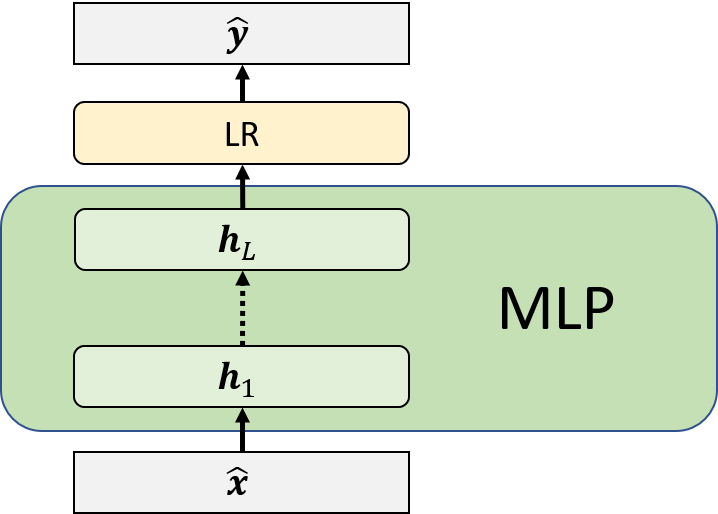
\includegraphics[width=\textwidth]{pics/dnn.png}
\caption{Deep Neural Network for Classification}\label{fig:dnn}
\end{minipage}
\begin{minipage}{.04\textwidth}
\end{minipage}
\begin{minipage}{.48\textwidth}
  \centering
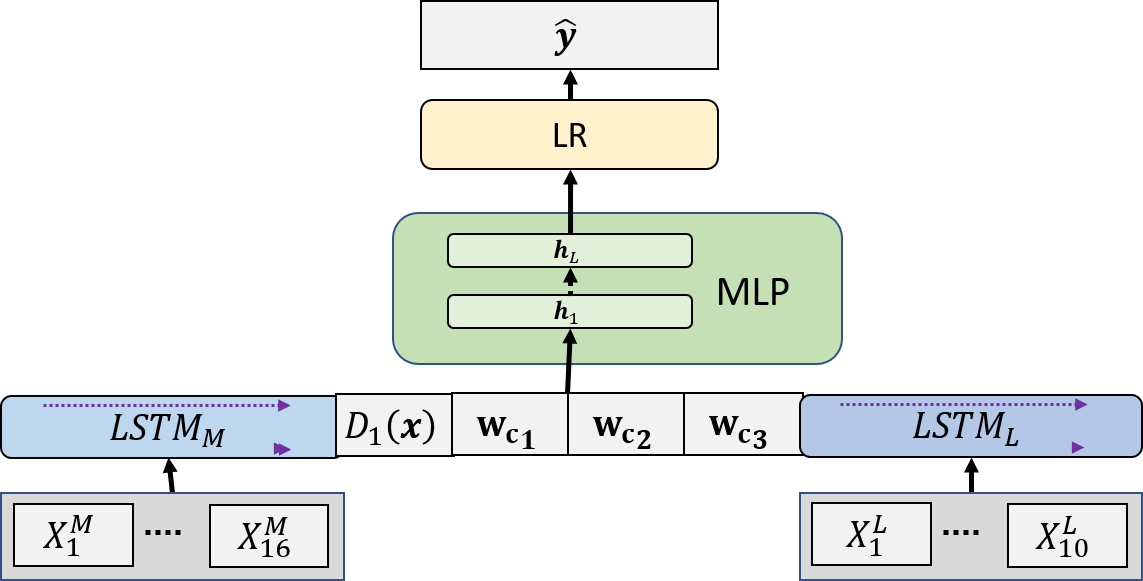
\includegraphics[width=\textwidth]{pics/rnn.png}
\caption{Recurrent Neural Network for Classification}\label{fig:rnn}
\end{minipage}
\end{figure}
%============================================================================================
% Subsection Experimental Setup================================================
%=============================================================================================
%============================================================================================
%============================================================================================
%Section: Results and Analysis================================================
%=============================================================================================
%============================================================================================
\section{Results and Analysis}
In this section we discuss the results of experiments and analyze the model predictions. % for the final mapping product. In section \ref{sec:res1} we discuss performance of all models trained for the field locations in the dataset. Following this discussion we perform a detailed ablation analysis for the described subsets of variables on the best performing model. To this end we first discuss training statistics for models from each variable subset, performing an ablation analysis on key training statistics. We then look more closely at the classification performance to assess potential weaknesses in the prospective model by analysis of predictions versus true class considering high level derived variables such as ecoregion, coverage class and soil regime. Finally, we shift our focus to analysis and assessment of the complete mapping product derived from the highest performing model, with specific focus on the variation of confidence for various points in the full study region that were not present in the training data. 
%============================================================================================
% Subsection Performance on Field measurement locations================================================
%=============================================================================================
\subsection{Performance on Field measurement locations}
In this section we report statistics on field measurement locations.
\subsubsection{Quantitative assessment} \label{sec:res1}
Quantitative results are reported for the average performance across cross-validation folds for each of the 4 subsets of input variables. Table \ref{tab:perf2} shows the outcomes of experiments in terms of accuracy for classification prediction. 
The best performing subset of input variables is bolded in each row of the tables, while the best overall performing model, the DNN using all available input data is highlighted in red. We note a a few trends. Incorporating satellite data of either form leads to better results. In addition, Random forest and LDA do not gain any advantage from incorporating both MODIS and LandSat imagery whereas the neural network models improve in accuracy from incorporating imagery from both platforms. Finally, we note that the recurrent neural network did not perform as well as the DNN, possibly due to the larger number of parameters to be fit on the same number of data points.

We chose the best performing model in terms of accuracy (DNN with all input variables) to create the final mapping product, and for this model we report several classification statistics for each of the four input variable subsets in Table \ref{tab:dnnperf}. Here we the same trend for recall, F-score, and area under the ROC curve in that adding imagery from either sattellite platform gives the most significant improvement, with the LandSat imagery demonstrating more improvement. The best results for all these metrics are once again from the inclusion of imagery from both satellite platforms.

 
\begin{table}
\begin{tabularx}{\linewidth}{l r r r r r r}
		\toprule[.2em]
		 &{\bf Prec.}& {\bf Rec.}&{\bf F-scr}&{\bf AUC}&{\bf Acc.}&{\bf Std.}\\
		\midrule
		$D_1$&0.755&0.820&0.768&0.825&0.767&0.021\\
		$D_2$&0.795&0.820&0.808&0.870&0.796&0.021\\
		$D_3$&0.818&0.832&0.822&0.887&0.812&0.019\\
		$D_4$&0.819& 0.827&0.822&0.889&0.814&0.012\\
		\bottomrule[.2em]
	\end{tabularx}
	\caption{Performance across a range of metrics for most accurate LR models for each subset of input variables. The last column reports the standard deviation of the accuracy across different cross-validation folds.} \label{tab:dnnperf}
\end{table}

\begin{figure}
  \begin{minipage}[b]{0.49\textwidth}
    \centering
 \begin{tabularx}{\linewidth}{l r r r r r}
		\toprule[.2em]
		 &$D_1$& $D_2$&$D_3$&$D_4$\\
		\midrule
		{\bf LR}&76.722&79.620&81.194&81.443\\
		{\bf LDA}&73.816 & 78.279&{\bf 80.653} &79.826\\
		{\bf RF}&80.165 &81.677&82.502 &{\bf 82.798}\\
		{\bf DNN}&79.604& 82.004&82.456 &\textcolor{red}{\bf 83.203}\\
		{\bf RNN}&--- & 82.050&82.580&{\bf 83.184}\\
		\bottomrule[.2em]
	\end{tabularx}
	\captionof{table}{Classification accuracy of models for subsets of data} \label{tab:perf2}
    \end{minipage}
\hfill
  \begin{minipage}[b]{0.49\textwidth}
    \centering
%\begin{tabularx}{\linewidth}{l r r r r r}
%		\toprule[.2em]
%		 &$D_1$ &$D_2$&$D_3$&$D_4$\\
%		\midrule
%		{\bf LR}&0.1340  & 0.1115&{\bf 0.1041} &0.1059\\
%		{\bf RF}& 0.0913  &0.0926&0.0909 &{\bf 0.0909}\\
%		{\bf DNN}&0.1006  &0.0795&0.0787 &\textcolor{red}{\bf 0.0746}\\
%		{\bf RNN}&---  & 0.0790&0.0806 &{\bf 0.0766}\\
%		\bottomrule[.2em]
%	\end{tabularx}
%	\captionof{table}{Mean Absolute Error for predicting cheat grass coverage.} \label{tab:perf3}
\begin{tabularx}{\linewidth}{l r r r r r r}
		\toprule[.2em]
		 &{\bf Prec.}& {\bf Rec.}&{\bf F-scr}&{\bf AUC}&{\bf Acc.}&{\bf Std.}\\
		\midrule
		$D_1$&0.795& 0.820&0.808 &0.866&0.796&0.025\\
		$D_2$&0.844 &0.803&0.823 &0.893&0.820&0.014\\
		$D_3$&0.831& 0.833&0.832 &0.900&0.825&0.015\\
		$D_4$&0.837& 0.842&0.839 &0.902&0.832&0.012\\
		\bottomrule[.2em]
	\end{tabularx}
	\captionof{table}{Performance across a range of metrics for most accurate DNN models for each subset of input variables. The last column reports the standard deviation of the accuracy across different cross-validation folds.} \label{tab:dnnperf}
  \end{minipage}
 
  \end{figure}

 \begin{figure}
  \begin{minipage}[b]{0.49\textwidth}
    \centering



\begin{tabularx}{\linewidth}{l r r r r r r}
		\toprule[.2em]
		 &{\bf Prec.}& {\bf Rec.}&{\bf F-scr}&{\bf AUC}&{\bf Acc.}&{\bf Std.}\\
		\midrule
		$D_1$&--& --&-- &--&--&--\\
		$D_2$&0.827&0.829&0.828&0.897&0.820&0.011\\
		$D_3$&0.829&0.841&0.835&0.901&0.827&0.012\\
		$D_4$&0.835& 0.844&0.840&0.906&0.832&0.012\\
		\bottomrule[.2em]
	\end{tabularx}
	\captionof{table}{Performance across a range of metrics for most accurate RNN models for each subset of input variables. The last column reports the standard deviation of the accuracy across different cross-validation folds.} \label{tab:dnnperf}
    \end{minipage}
\hfill
  \begin{minipage}[b]{0.49\textwidth}
    \centering




\begin{tabularx}{\linewidth}{l r r r r r r}
		\toprule[.2em]
		 &{\bf Prec.}& {\bf Rec.}&{\bf F-scr}&{\bf AUC}&{\bf Acc.}&{\bf Std.}\\
		\midrule
		$D_1$&0.807& 0.815&0.811 &0.883&0.802&0.024\\
		$D_2$&0.825 &0.823&0.824 &0.891&0.816&0.024\\
		$D_3$&0.827& 0.838&0.833 &0.901&0.825&0.021\\
		$D_4$&0.835& 0.835&0.835 &0.904&0.828&0.025\\
		\bottomrule[.2em]
	\end{tabularx}
	\captionof{table}{Performance across a range of metrics for most accurate RF models for each subset of input variables. The last column reports the standard deviation of the accuracy across different cross-validation folds.} \label{tab:dnnperf}
  \end{minipage}
 
  \end{figure}
%\begin{table}
%\begin{tabularx}{\linewidth}{l r r r r r r}
%		\toprule[.2em]
%		 &{\bf Precision}& {\bf Recall}&{\bf F-score}&{\bf AUC}&{\bf Accuracy}&{\bf Std. Accuracy}\\
%		\midrule
%		$D_1$&0.795& 0.820&0.808 &0.866&0.796&0.025\\
%		$D_2$&0.844 &0.803&0.823 &0.893&0.820&0.014\\
%		$D_3$&0.831& 0.833&0.832 &0.900&0.825&0.015\\
%		$D_4$&0.837& 0.842&0.839 &0.902&0.832&0.012\\
%		\bottomrule[.2em]
%	\end{tabularx}
%	\caption{Performance across a range of metrics for most accurate DNN models for each subset of input variables.} \label{tab:dnnperf}
%\end{table}

%================================
% Subsubsection Training Statistics
%================================
\subsubsection{Training Statistics}
In this section we analyse training statistics for the best performing model. We first look at plots of train versus test performance for the best performing cross-validation fold for each of the input variable subsets. Looking at several different metrics we see training is noisier and has a greater tendency to overfit with inclusion of the modis data. Conversely we see that incorporating the LandSat data into the model has a regularizing effect which limits the amount of overfitting so that test performance converges closer to train performance. We also consider the dropout probability for each data subset (for each model run a random dropout probability was selected to be between 0.5 and 1.0. Table \ref{drop} shows the dropout probabilities and hidden layer sizes for the different data subsets. The columns for using MODIS only or LandSat show that these models have comparable dropout probabilities and network size. The MODIS only input model does have the largest network which greatens the chance of overfitting but a large dropout probability which should have more of a regularizing effect. A more careful analysis with identical sized networks and dropout probabilities would confirm what the present analysis suggests (that the MODIS data has some properties which encourage overfitting). With careful use of early stopping we can see in figure 53 that the best loss  can in fact be achieved by incorporating all the data. 

\begin{table}
\begin{tabularx}{\linewidth}{l r r r r}
		\toprule[.2em]
		 &{\bf $D_1$}& {\bf $D_2$}&{\bf $D_3$}&{\bf $D_4$}\\
		\midrule
		Dropout Probability&0.275&0.350& 0.30&.5\\
		Layer 1&256&256& 256&256\\
		Layer 2&256&256&64&32\\
		Layer 3&64&128&256&256\\
		\bottomrule[.2em]
	\end{tabularx}
	\caption{Hyperparameters for most accurate DNN models for each subset of input variables.} \label{tab:dnnhyper}
\end{table}
%d1 dp 7.25 256 256 64
%d2 dp 0.65 256 256 128
%d3 dp 0.7 256 64 256
%d4 dp .5 256 32 256
%================================
% Subsubsection Best Training Statistics
%================================
% Accuracy Train versus test
%best
%\begin{figure}
%\centering
%\begin{minipage}{.24\textwidth}
%  \centering
%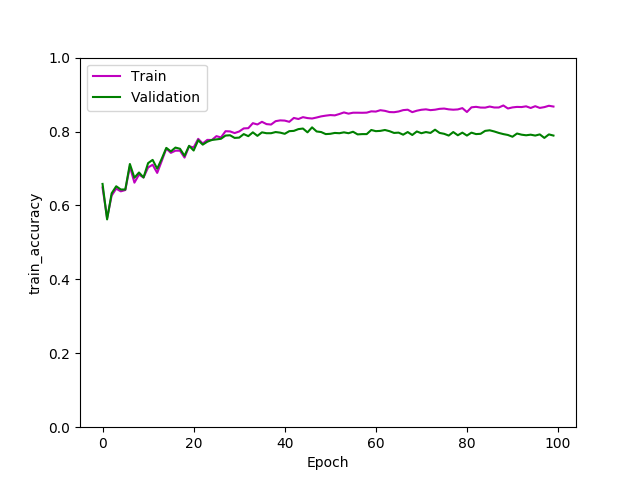
\includegraphics[width=\textwidth]{pics/d1_train_accuracy_best_train_test.png}
%\caption{$D_1$}\label{fig:d1acctraintest}
%\end{minipage}
%\begin{minipage}{.01\textwidth}
%\end{minipage}
%\begin{minipage}{.24\textwidth}
%  \centering
%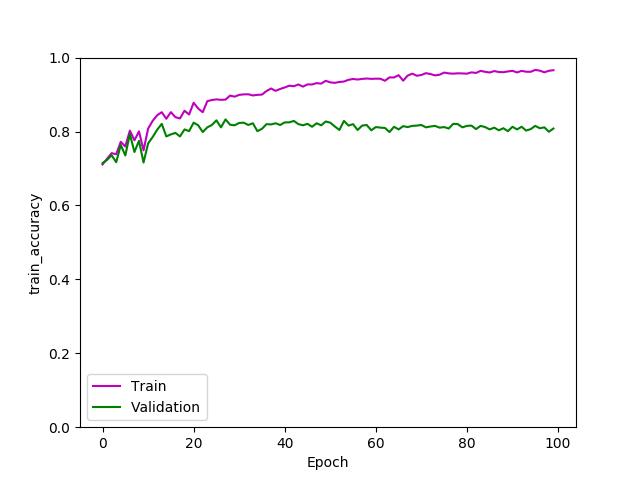
\includegraphics[width=\textwidth]{pics/d2_train_accuracy_best_train_test.png}
%\caption{$D_2$}\label{fig:d2acctraintest}
%\end{minipage}
%\begin{minipage}{.24\textwidth}
%  \centering
%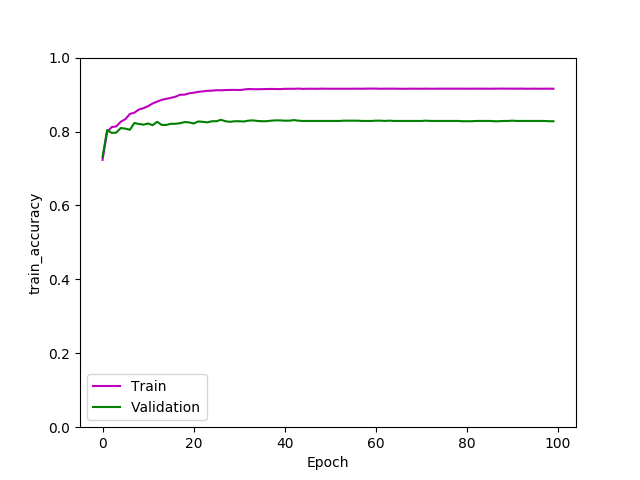
\includegraphics[width=\textwidth]{pics/d3_train_accuracy_best_train_test.png}
%\caption{$D_3$}\label{fig:d3acctraintest}
%\end{minipage}
%\begin{minipage}{.01\textwidth}
%\end{minipage}
%% average
%\begin{minipage}{.24\textwidth}
%  \centering
%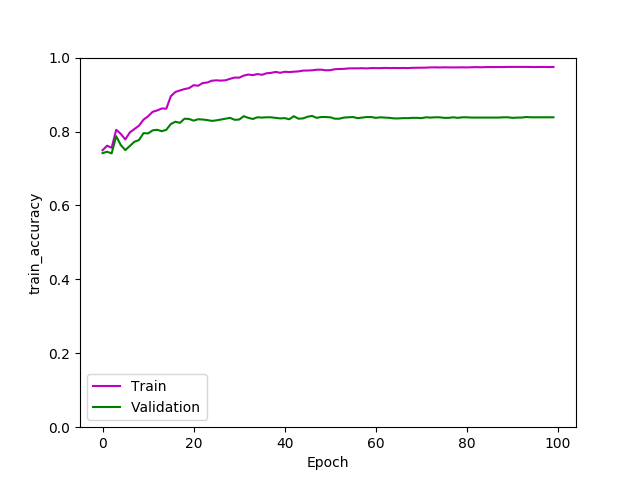
\includegraphics[width=\textwidth]{pics/d4_train_accuracy_best_train_test.png}
%\caption{$D_4$}\label{fig:d4acctraintest}
%\end{minipage}
%\caption{Train versus test accuracy for the best performing cross-validation fold for input variable subsets}\label{fig:traintestacc}
%\end{figure}
%\begin{figure}
%\centering
%\begin{minipage}{.24\textwidth}
%  \centering
%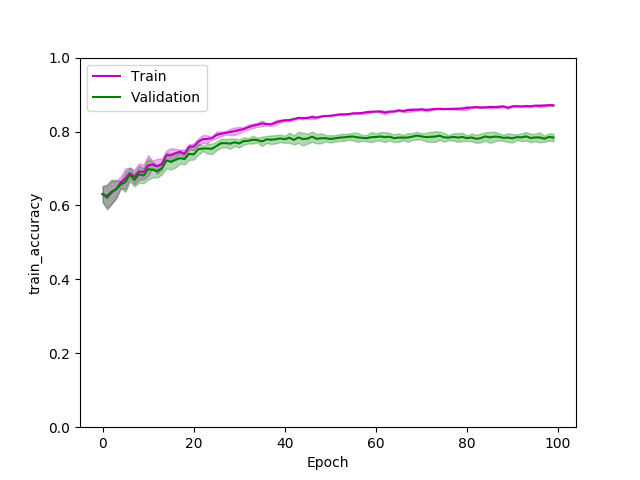
\includegraphics[width=\textwidth]{pics/d1_train_accuracy_mean_train_test.png}
%\caption{$D_1$}\label{fig:d1acctraintest}
%\end{minipage}
%\begin{minipage}{.01\textwidth}
%\end{minipage}
%\begin{minipage}{.24\textwidth}
%  \centering
%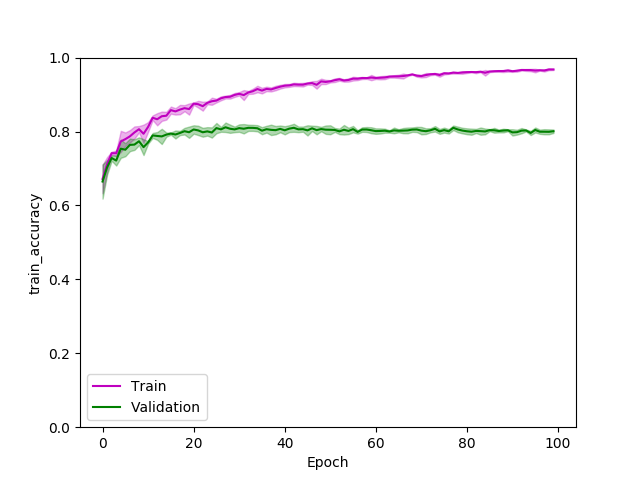
\includegraphics[width=\textwidth]{pics/d2_train_accuracy_mean_train_test.png}
%\caption{$D_2$}\label{fig:d2acctraintest}
%\end{minipage}
%\begin{minipage}{.24\textwidth}
%  \centering
%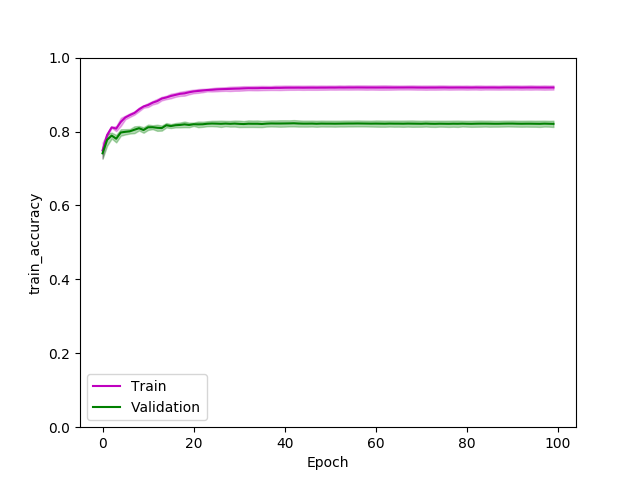
\includegraphics[width=\textwidth]{pics/d3_train_accuracy_mean_train_test.png}
%\caption{$D_3$}\label{fig:d3acctraintest}
%\end{minipage}
%\begin{minipage}{.01\textwidth}
%\end{minipage}
%\begin{minipage}{.24\textwidth}
%  \centering
%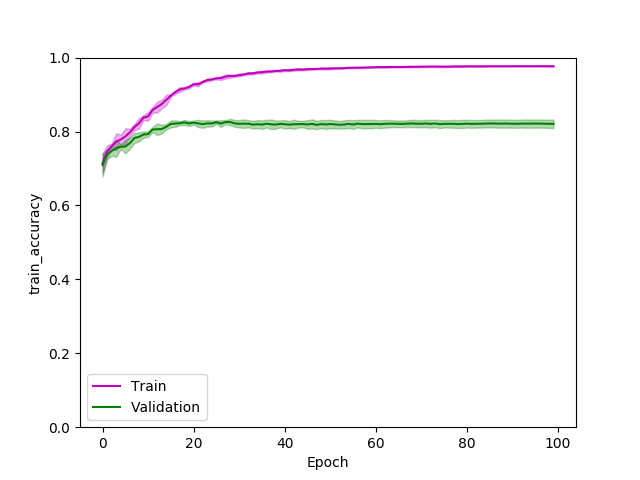
\includegraphics[width=\textwidth]{pics/d4_train_accuracy_mean_train_test.png}
%\caption{$D_4$}\label{fig:d4acctraintest}
%\end{minipage}
%\caption{Train versus test accuracy for the average of cross-validation folds for input variable subsets}\label{fig:traintestacc}
%\end{figure}
%% ROC Train versus test
%%best
%\begin{figure}
%\centering
%\begin{minipage}{.24\textwidth}
%  \centering
%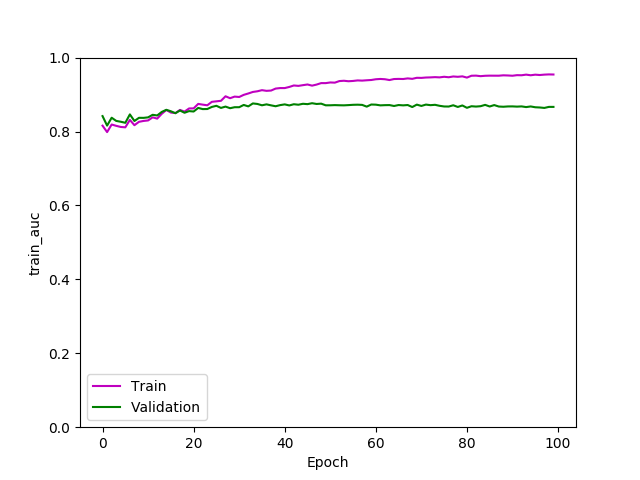
\includegraphics[width=\textwidth]{pics/d1_train_auc_best_train_test.png}
%\caption{$D_1$}\label{fig:d1acctraintest}
%\end{minipage}
%\begin{minipage}{.01\textwidth}
%\end{minipage}
%\begin{minipage}{.24\textwidth}
%  \centering
%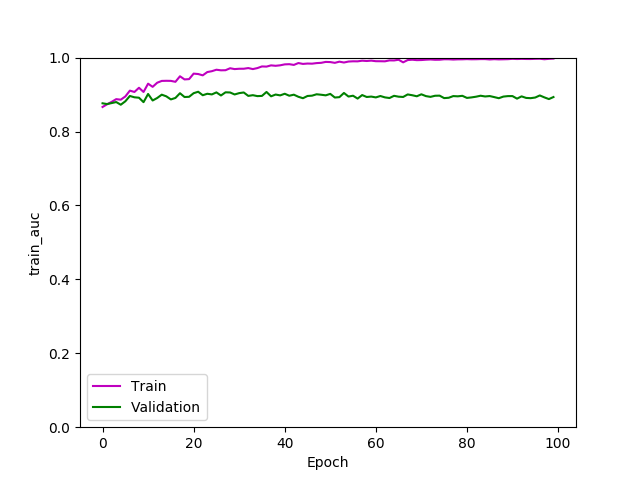
\includegraphics[width=\textwidth]{pics/d2_train_auc_best_train_test.png}
%\caption{$D_2$}\label{fig:d2acctraintest}
%\end{minipage}
%\begin{minipage}{.24\textwidth}
%  \centering
%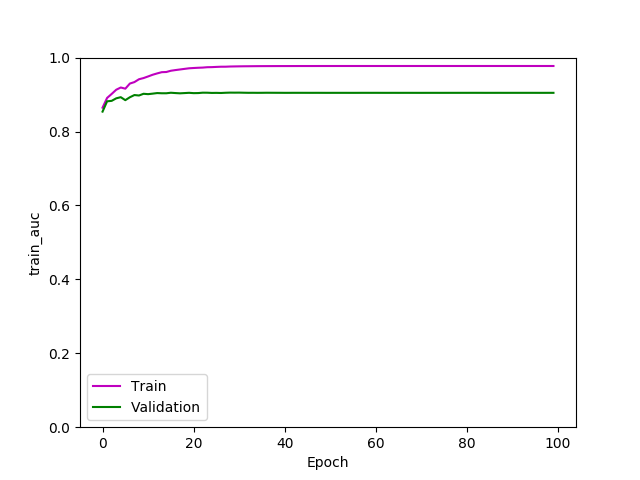
\includegraphics[width=\textwidth]{pics/d3_train_auc_best_train_test.png}
%\caption{$D_3$}\label{fig:d3acctraintest}
%\end{minipage}
%\begin{minipage}{.01\textwidth}
%\end{minipage}
%\begin{minipage}{.24\textwidth}
%  \centering
%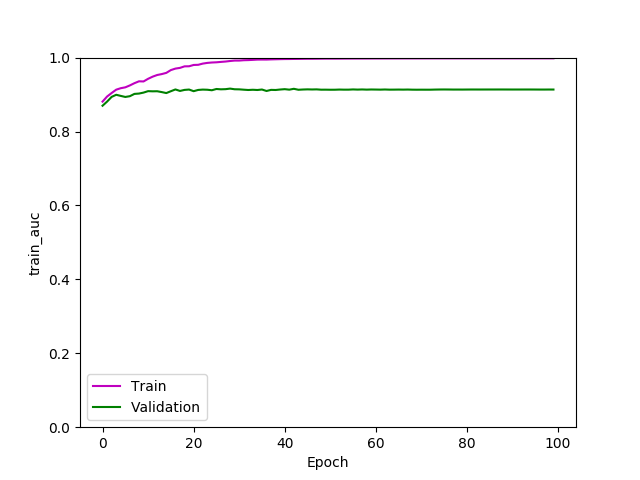
\includegraphics[width=\textwidth]{pics/d4_train_auc_best_train_test.png}
%\caption{$D_4$}\label{fig:d4acctraintest}
%\end{minipage}
%\caption{Train versus test area under the ROC curve for best performing cross-validation fold for input variable subsets}\label{fig:traintestauc}
%\end{figure}
%%average
%\begin{figure}
%\centering
%\begin{minipage}{.24\textwidth}
%  \centering
%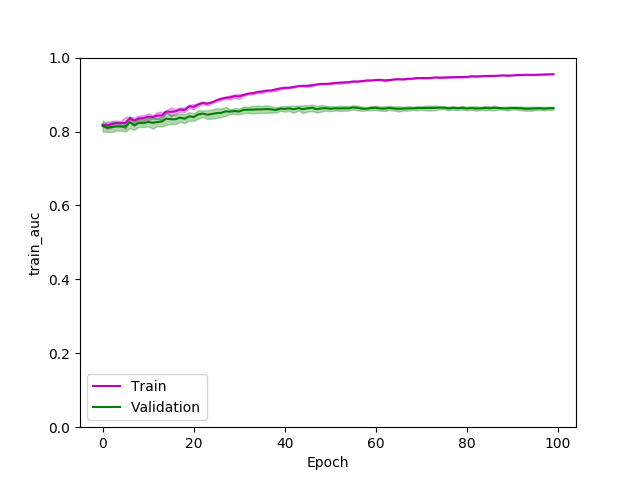
\includegraphics[width=\textwidth]{pics/d1_train_auc_mean_train_test.png}
%\caption{$D_1$}\label{fig:d1acctraintest}
%\end{minipage}
%\begin{minipage}{.01\textwidth}
%\end{minipage}
%\begin{minipage}{.24\textwidth}
%  \centering
%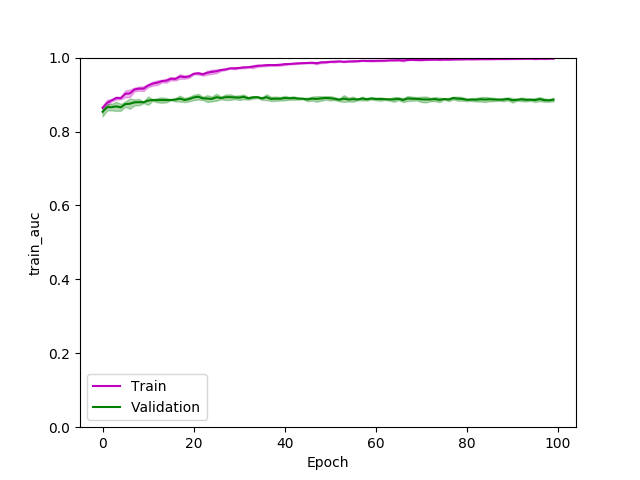
\includegraphics[width=\textwidth]{pics/d2_train_auc_mean_train_test.png}
%\caption{$D_2$}\label{fig:d2acctraintest}
%\end{minipage}
%\begin{minipage}{.24\textwidth}
%  \centering
%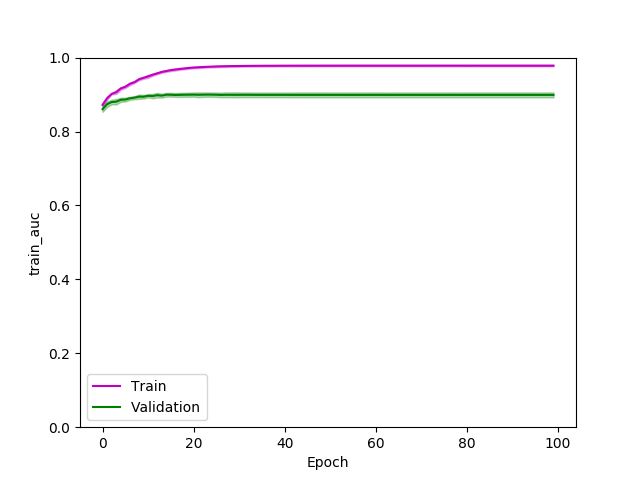
\includegraphics[width=\textwidth]{pics/d3_train_auc_mean_train_test.png}
%\caption{$D_3$}\label{fig:d3acctraintest}
%\end{minipage}
%\begin{minipage}{.01\textwidth}
%\end{minipage}
%\begin{minipage}{.24\textwidth}
%  \centering
%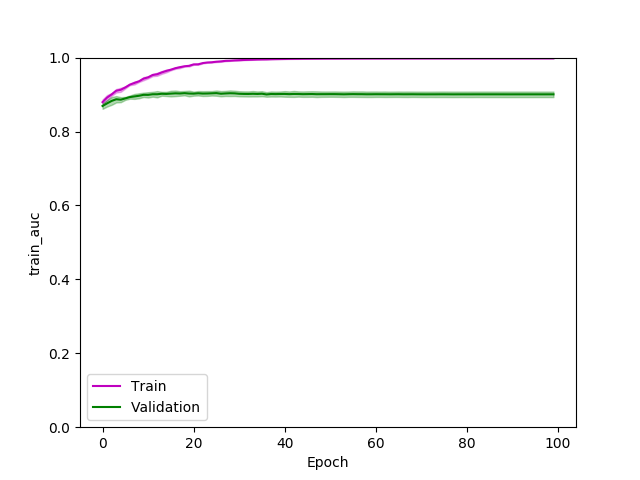
\includegraphics[width=\textwidth]{pics/d4_train_auc_mean_train_test.png}
%\caption{$D_4$}\label{fig:d4acctraintest}
%\end{minipage}
%\caption{Train versus test area under the ROC curve for average of cross-validation folds for input variable subsets}\label{fig:traintestauc}
%\end{figure}
%% F-measure Train versus test
%%best
%\begin{figure}
%\centering
%\begin{minipage}{.24\textwidth}
%  \centering
%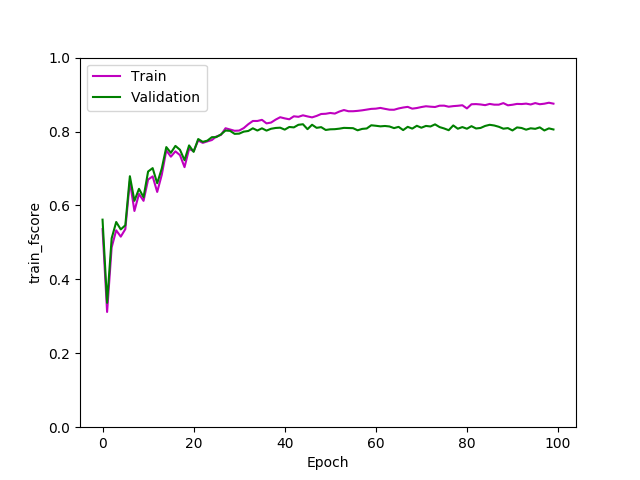
\includegraphics[width=\textwidth]{pics/d1_train_fscore_best_train_test.png}
%\caption{$D_1$}\label{fig:d1fscoretraintest}
%\end{minipage}
%\begin{minipage}{.01\textwidth}
%\end{minipage}
%\begin{minipage}{.24\textwidth}
%  \centering
%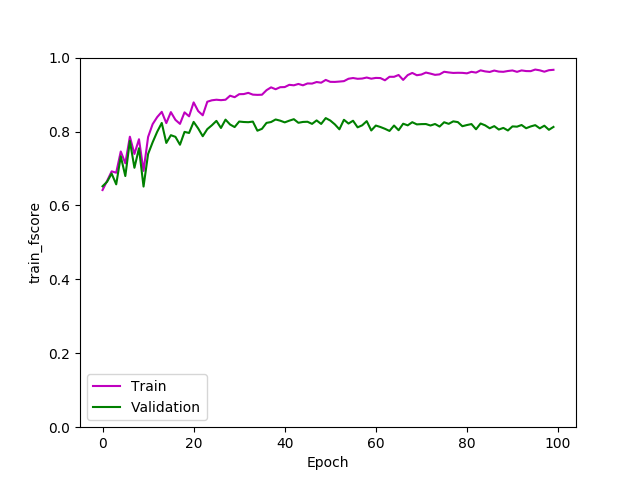
\includegraphics[width=\textwidth]{pics/d2_train_fscore_best_train_test.png}
%\caption{$D_2$}\label{fig:d2fscoretraintest}
%\end{minipage}
%\begin{minipage}{.24\textwidth}
%  \centering
%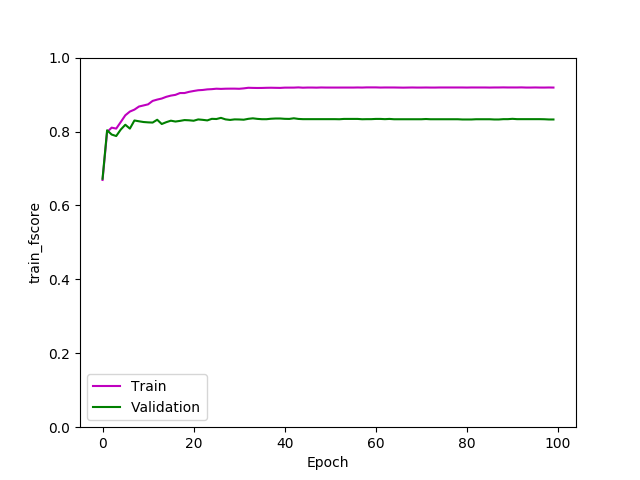
\includegraphics[width=\textwidth]{pics/d3_train_fscore_best_train_test.png}
%\caption{$D_3$}\label{fig:d3fscoretraintest}
%\end{minipage}
%\begin{minipage}{.01\textwidth}
%\end{minipage}
%\begin{minipage}{.24\textwidth}
%  \centering
%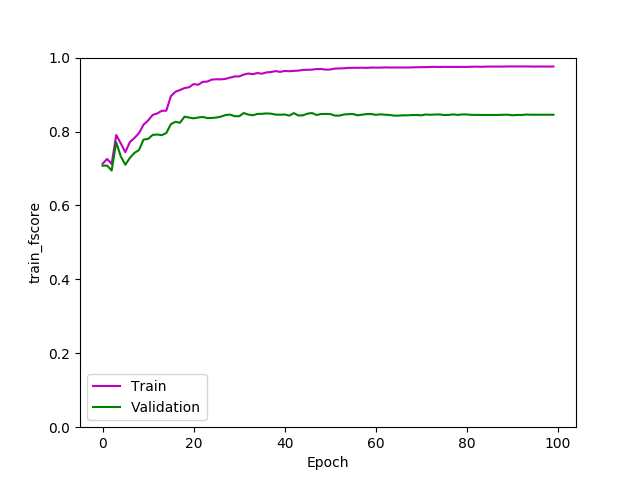
\includegraphics[width=\textwidth]{pics/d4_train_fscore_best_train_test.png}
%\caption{$D_4$}\label{fig:d4fscoretraintest}
%\end{minipage}
%\caption{Train versus test F-score of best performing cross-validation fold for input variable subsets}\label{fig:traintestfscore}
%\end{figure}
%%average
%\begin{figure}
%\centering
%\begin{minipage}{.24\textwidth}
%  \centering
%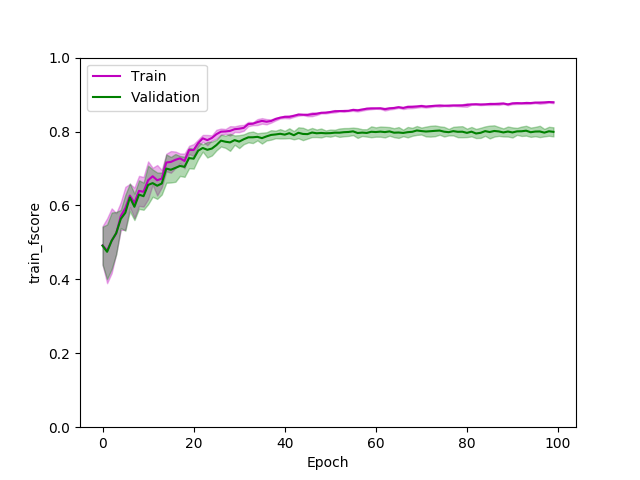
\includegraphics[width=\textwidth]{pics/d1_train_fscore_mean_train_test.png}
%\caption{$D_1$}\label{fig:d1fscoretraintest}
%\end{minipage}
%\begin{minipage}{.01\textwidth}
%\end{minipage}
%\begin{minipage}{.24\textwidth}
%  \centering
%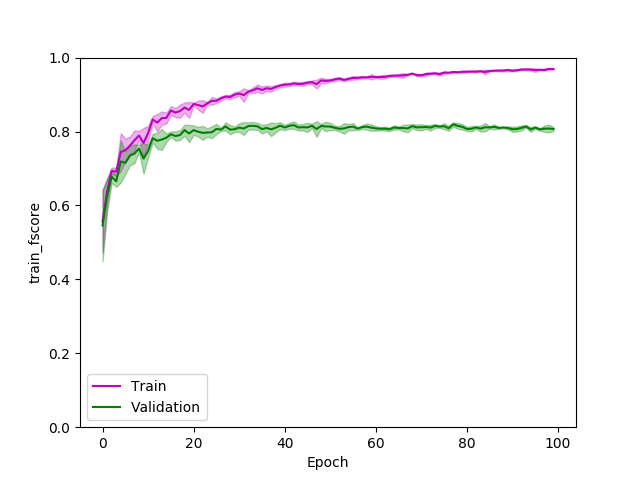
\includegraphics[width=\textwidth]{pics/d2_train_fscore_mean_train_test.png}
%\caption{$D_2$}\label{fig:d2fscoretraintest}
%\end{minipage}
%\begin{minipage}{.24\textwidth}
%  \centering
%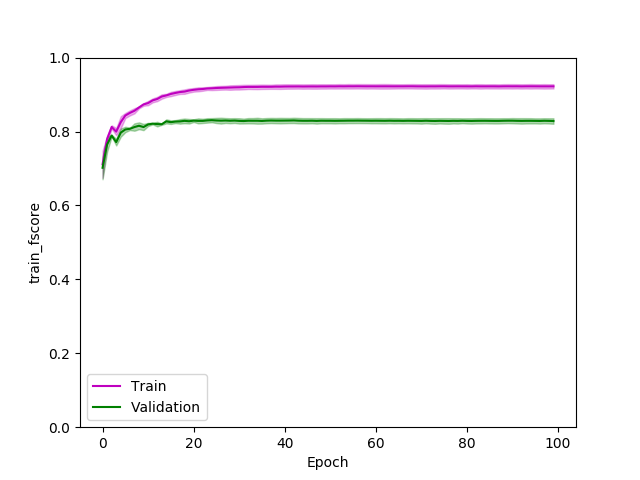
\includegraphics[width=\textwidth]{pics/d3_train_fscore_mean_train_test.png}
%\caption{$D_3$}\label{fig:d3fscoretraintest}
%\end{minipage}
%\begin{minipage}{.01\textwidth}
%\end{minipage}
%\begin{minipage}{.24\textwidth}
%  \centering
%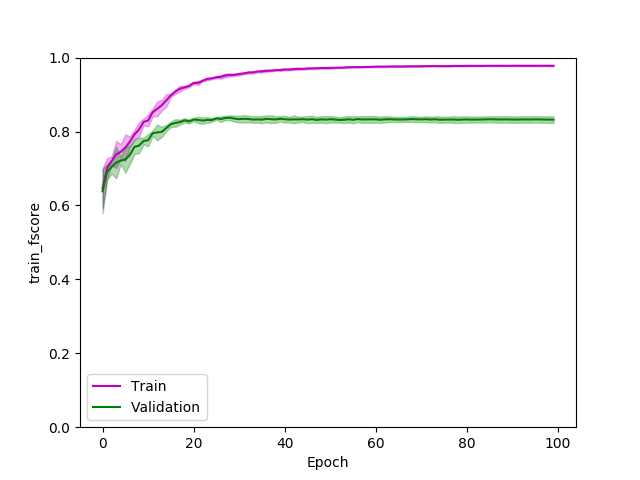
\includegraphics[width=\textwidth]{pics/d4_train_fscore_mean_train_test.png}
%\caption{$D_4$}\label{fig:d4fscoretraintest}
%\end{minipage}
%\caption{Train versus test F-score of average cross-validation score for input variable subsets}\label{fig:traintestfscore}
%\end{figure}
%% Cross Entropy Train versus test
%%best
%\begin{figure}
%\centering
%\begin{minipage}{.24\textwidth}
%  \centering
%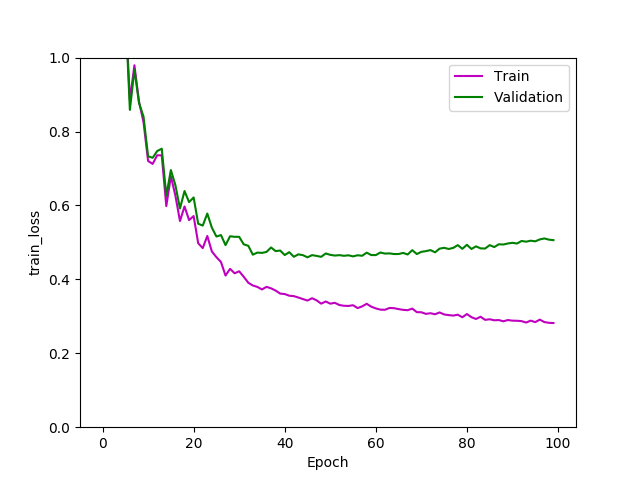
\includegraphics[width=\textwidth]{pics/d1_train_loss_best_train_test.png}
%\caption{$D_1$}\label{fig:d1lossraintest}
%\end{minipage}
%\begin{minipage}{.01\textwidth}
%\end{minipage}
%\begin{minipage}{.24\textwidth}
%  \centering
%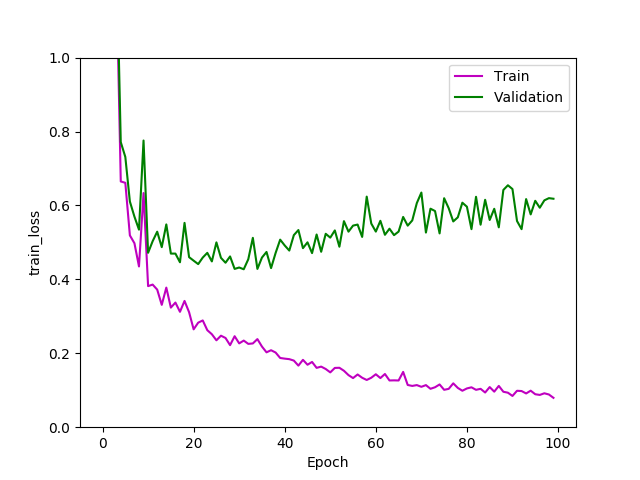
\includegraphics[width=\textwidth]{pics/d2_train_loss_best_train_test.png}
%\caption{$D_2$}\label{fig:d2losstraintest}
%\end{minipage}
%\begin{minipage}{.24\textwidth}
%  \centering
%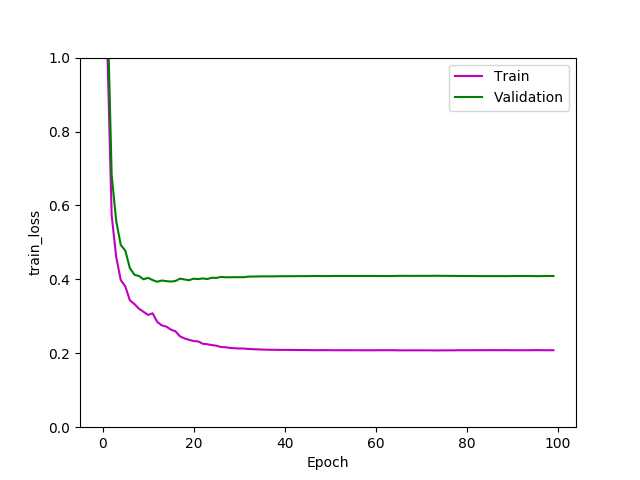
\includegraphics[width=\textwidth]{pics/d3_train_loss_best_train_test.png}
%\caption{$D_3$}\label{fig:d3losstraintest}
%\end{minipage}
%\begin{minipage}{.01\textwidth}
%\end{minipage}
%\begin{minipage}{.24\textwidth}
%  \centering
%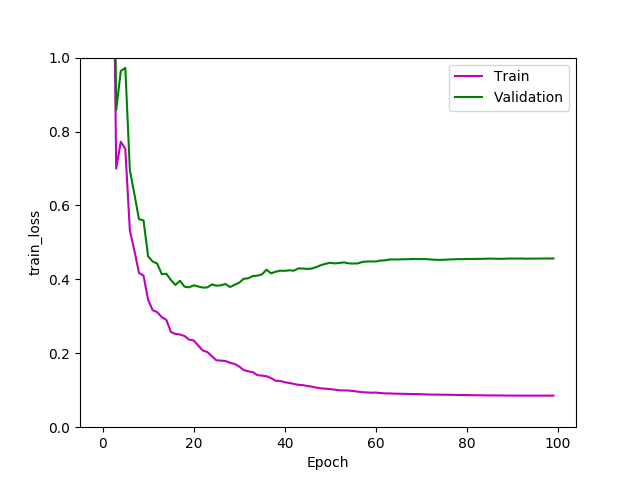
\includegraphics[width=\textwidth]{pics/d4_train_loss_best_train_test.png}
%\caption{$D_4$}\label{fig:d4losstraintest}
%\end{minipage}
%\caption{Train versus test cross entropy loss for best performing cross-validation fold for input variable subsets}\label{fig:traintesloss}
%\end{figure}
%%average
%\begin{figure}
%\centering
%\begin{minipage}{.24\textwidth}
%  \centering
%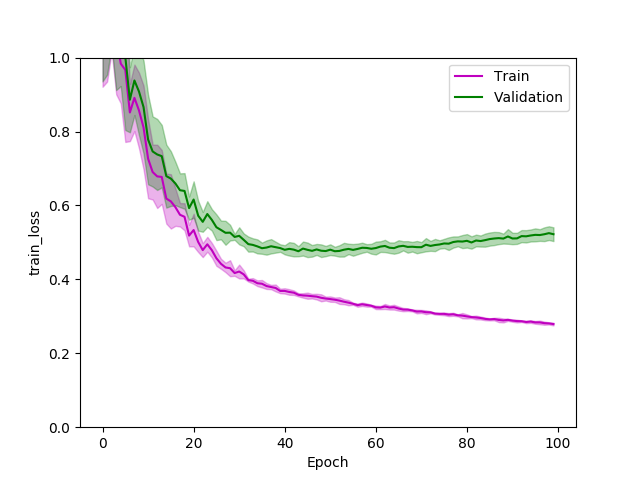
\includegraphics[width=\textwidth]{pics/d1_train_loss_mean_train_test.png}
%\caption{$D_1$}\label{fig:d1lossraintest}
%\end{minipage}
%\begin{minipage}{.01\textwidth}
%\end{minipage}
%\begin{minipage}{.24\textwidth}
%  \centering
%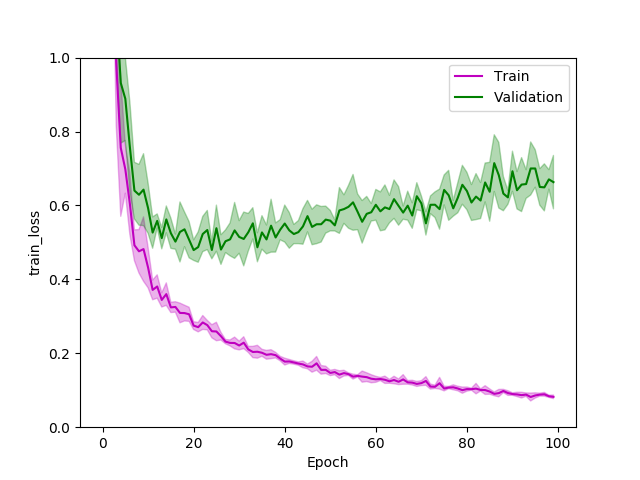
\includegraphics[width=\textwidth]{pics/d2_train_loss_mean_train_test.png}
%\caption{$D_2$}\label{fig:d2losstraintest}
%\end{minipage}
%\begin{minipage}{.24\textwidth}
%  \centering
%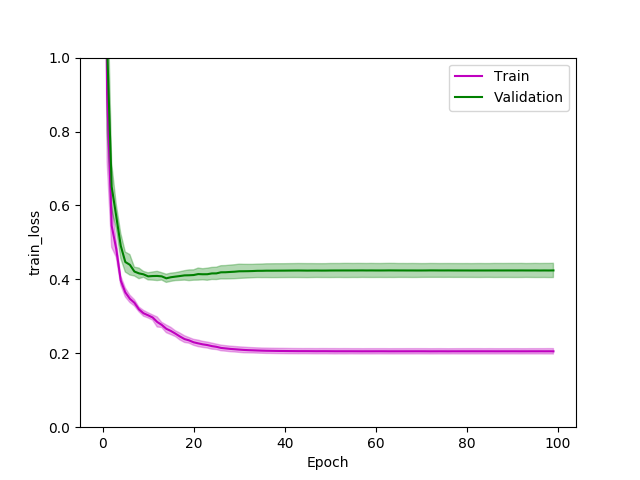
\includegraphics[width=\textwidth]{pics/d3_train_loss_mean_train_test.png}
%\caption{$D_3$}\label{fig:d3losstraintest}
%\end{minipage}
%\begin{minipage}{.01\textwidth}
%\end{minipage}
%\begin{minipage}{.24\textwidth}
%  \centering
%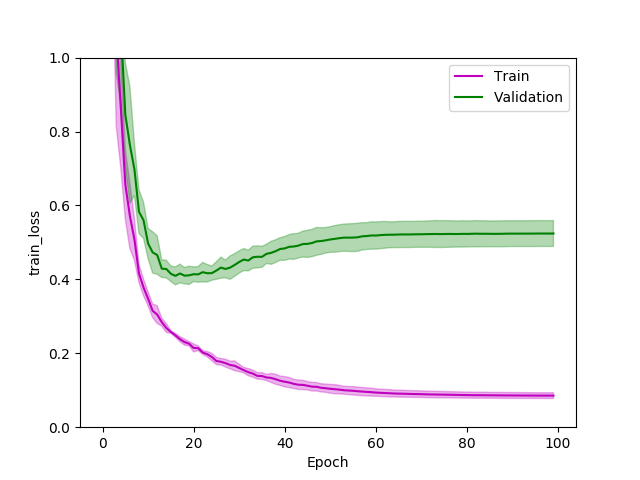
\includegraphics[width=\textwidth]{pics/d4_train_loss_mean_train_test.png}
%\caption{$D_4$}\label{fig:d4losstraintest}
%\end{minipage}
%\caption{Train versus test cross entropy loss for average of cross-validation folds for input variable subsets}\label{fig:traintesloss}
%\end{figure}
%%================================
%% Subsubsection Test performance comparisons across variable partitions
%%================================
%% Metrics on test
%% best
%\begin{figure}
%\centering
%\begin{minipage}{.24\textwidth}
%  \centering
%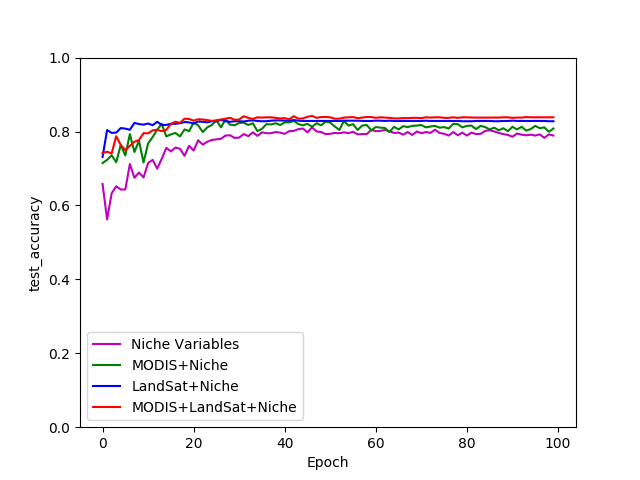
\includegraphics[width=\textwidth]{pics/test_accuracy_variables.png}
%\caption{Accuracy}\label{fig:subsetacc}
%\end{minipage}
%\begin{minipage}{.01\textwidth}
%\end{minipage}
%\begin{minipage}{.24\textwidth}
%  \centering
%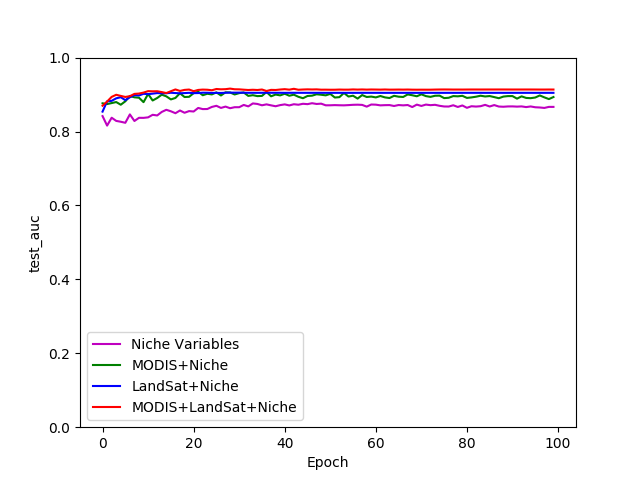
\includegraphics[width=\textwidth]{pics/test_auc_variables.png}
%\caption{Area under ROC}\label{fig:subsetauc}
%\end{minipage}
%\begin{minipage}{.24\textwidth}
%  \centering
%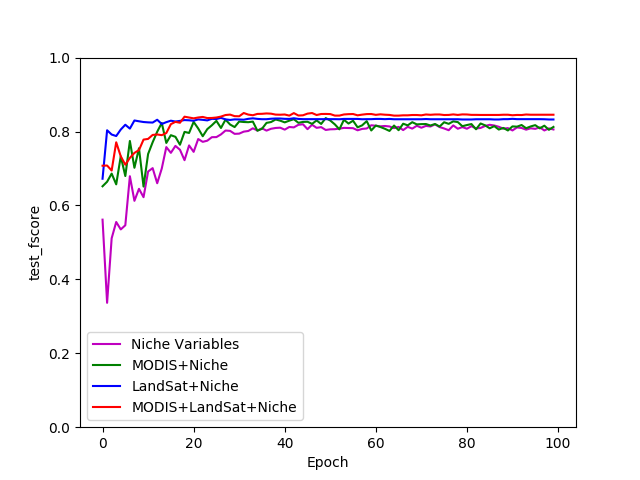
\includegraphics[width=\textwidth]{pics/test_fscore_variables.png}
%\caption{F-score}\label{fig:subsetfscore}
%\end{minipage}
%\begin{minipage}{.01\textwidth}
%\end{minipage}
%\begin{minipage}{.24\textwidth}
%  \centering
%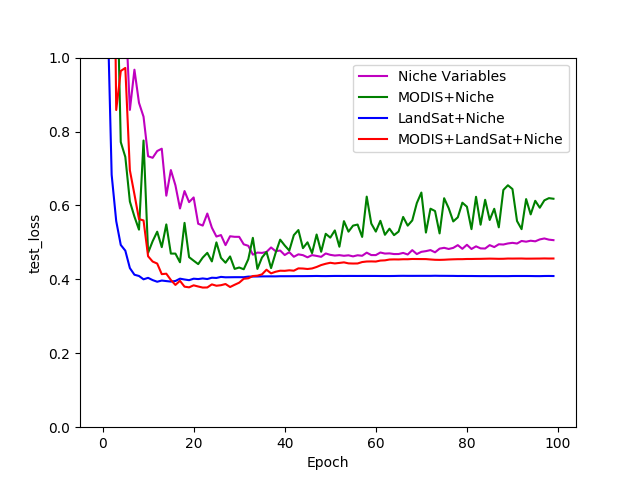
\includegraphics[width=\textwidth]{pics/test_loss_variables.png}
%\caption{Cross-entropy}\label{fig:subsetloss}
%\end{minipage}
%\caption{Test metrics plotted for input variable subsets}\label{fig:testmetrics}
%\end{figure}
%% average
%\begin{figure}
%\centering
%\begin{minipage}{.24\textwidth}
%  \centering
%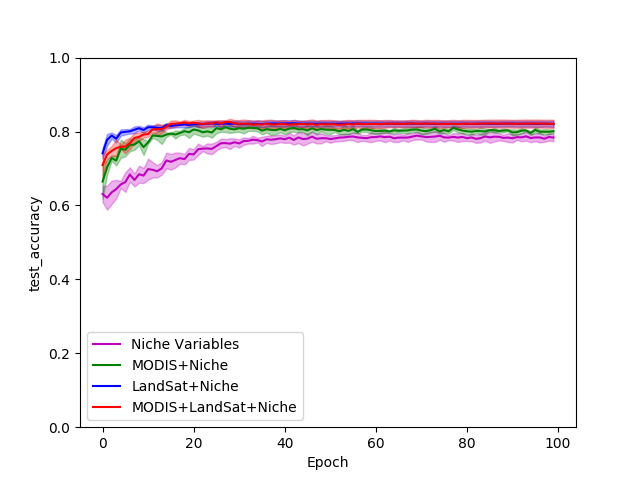
\includegraphics[width=\textwidth]{pics/test_accuracy_mean_variables.png}
%\caption{Accuracy}\label{fig:subsetacc}
%\end{minipage}
%\begin{minipage}{.01\textwidth}
%\end{minipage}
%\begin{minipage}{.24\textwidth}
%  \centering
%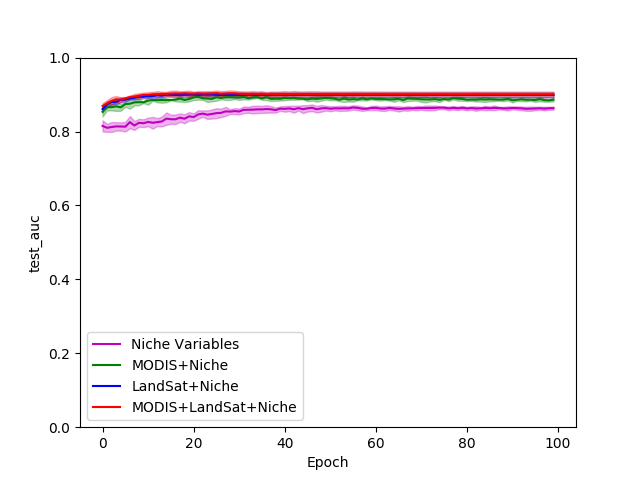
\includegraphics[width=\textwidth]{pics/test_auc_mean_variables.png}
%\caption{Area under ROC}\label{fig:subsetauc}
%\end{minipage}
%\begin{minipage}{.24\textwidth}
%  \centering
%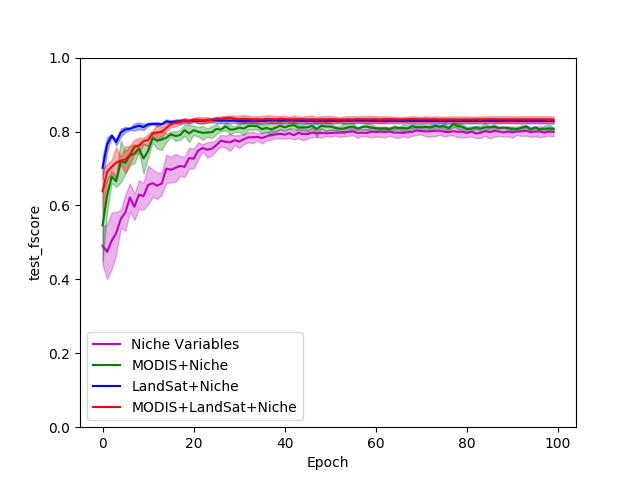
\includegraphics[width=\textwidth]{pics/test_fscore_mean_variables.png}
%\caption{F-score}\label{fig:subsetfscore}
%\end{minipage}
%\begin{minipage}{.01\textwidth}
%\end{minipage}
%\begin{minipage}{.24\textwidth}
%  \centering
%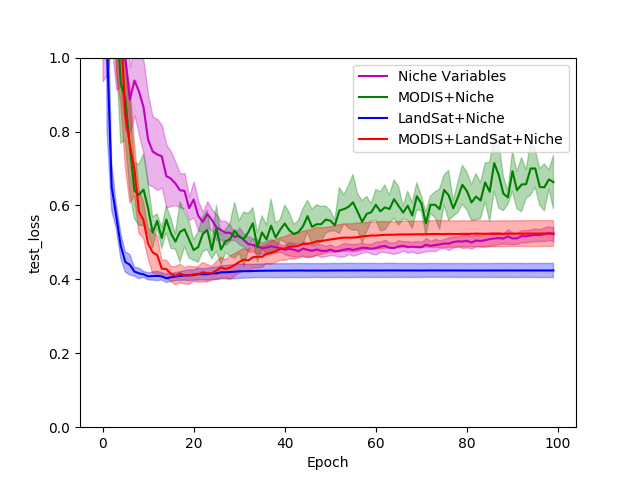
\includegraphics[width=\textwidth]{pics/test_loss_mean_variables.png}
%\caption{Cross-entropy}\label{fig:subsetloss}
%\end{minipage}
%\caption{Test metrics plotted for input variable subsets}\label{fig:testmetrics}
%\end{figure}
%================================
% Subsubsection Qualitative assessment
%================================
\subsubsection{Qualitative assesment}
In this section we characterize the overall performance of the best performing DNN models. Figure \ref{confusion} shows a confusion matrix for classification for the best performing DNN model using all the input variables. The types of mistakes the model makes in classification are evenly balanced in terms of false positives and false negatives, however since a smaller proportion of the data contains negative examples it in fact slightly favors false positives. We can see this more clearly in figure 63 which plots accuracy in terms of actual cheat grass coverage values. The worst performance is in the 0-2 percent range which contains only negative examples, so the only mistake that can be made is a false positive. 

Looking closer at prediction performance
we next analyze the model  in terms of accuracy across individual ranges of cheatgrass coverage, ecoregions, land cover classes, and soil and climactic conditions. 
Figures 60-61 show that the models incorporating the LandSat data attain 100 \% accuracy for actual coverage ranging from 70-100 \% cheat grass coverage and accuracy above 90 \% up down to 40 \% coverage. This is despite the fact that there are fewer examples in the data set for these high coverage locations. Since the overwhelming majority of false positives and false negatives fall within the 0-40 \% range, this suggests that changing the class boundary from 2\% to 40\% may lead to more accurate classification at the expense of the overall utility of a final mapping product.
We pay particular interest in judging if the model performs better across different ecoregions due to an unbalanced representation in the data set or something intrinsic in the environment itself.  
Across the other ways of splitting the data into ecoregion, soil moisture temperature regime, and land cover class we see that accuracy is not correlated with frequency of occurrence. Although there does seem to be a minimum threshold for number of examples for an ecoregion to attain acceptable accuracy, considering the low performance of ecoregions 25 and 16 and corresponding small number of examples.  


\begin{itemize}
\item{Map of field data symbolized by classification error}
\end{itemize}
% cheatgrass coverage versus accuracy
% average
\begin{figure}
\centering
\begin{minipage}{.24\textwidth}
  \centering
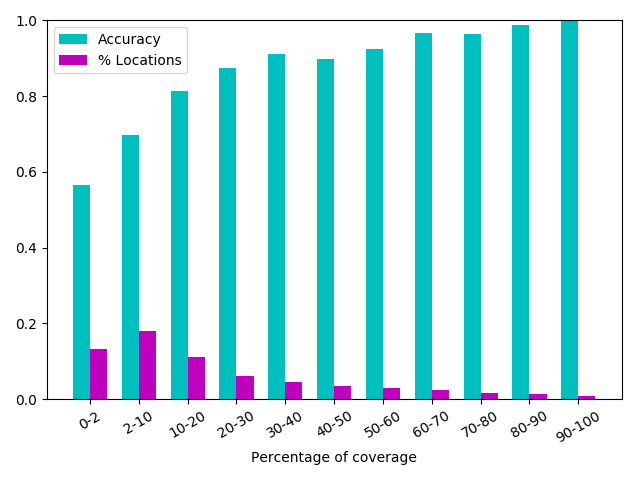
\includegraphics[width=\textwidth]{pics/d1_accuracy_vs_coverage.png}
\caption{$D_1$}
\end{minipage}
\begin{minipage}{.01\textwidth}
\end{minipage}
\begin{minipage}{.24\textwidth}
  \centering
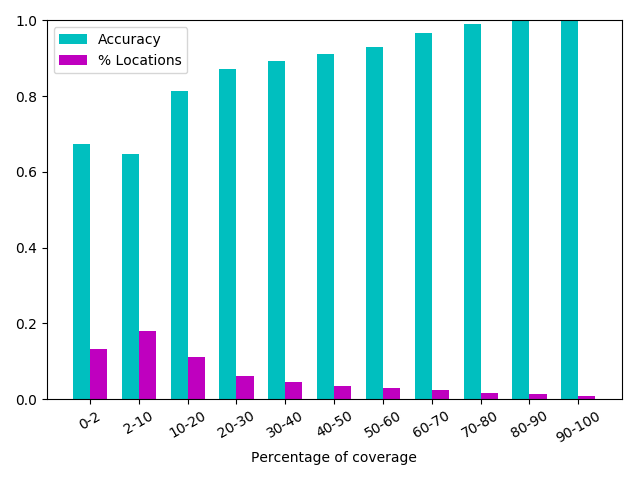
\includegraphics[width=\textwidth]{pics/d2_accuracy_vs_coverage.png}
\caption{$D_2$}
\end{minipage}
\begin{minipage}{.24\textwidth}
  \centering
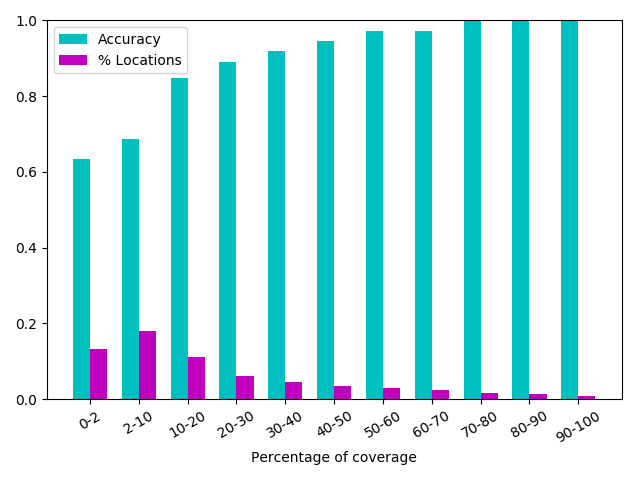
\includegraphics[width=\textwidth]{pics/d3_accuracy_vs_coverage.png}
\caption{$D_3$}
\end{minipage}
\begin{minipage}{.01\textwidth}
\end{minipage}
\begin{minipage}{.24\textwidth}
  \centering
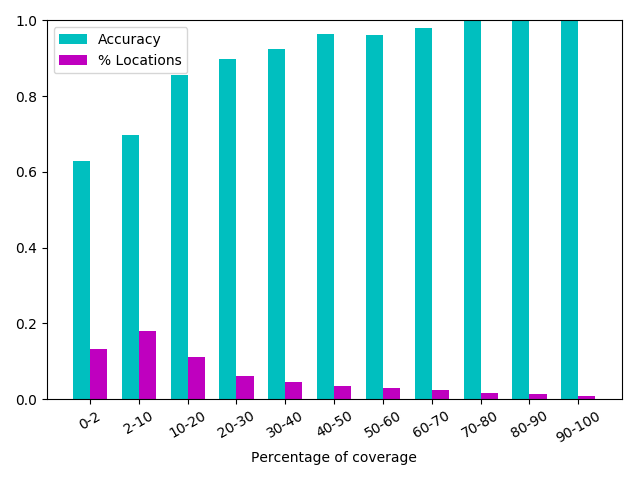
\includegraphics[width=\textwidth]{pics/d4_accuracy_vs_coverage.png}
\caption{$D_4$}
\end{minipage}
\caption{Accuracy for ranges of cheat grass coverage.}\label{fig:testmetrics}
\end{figure}
% accuracy versus categories
% average
\begin{figure}
\centering
\begin{minipage}{.24\textwidth}
  \centering
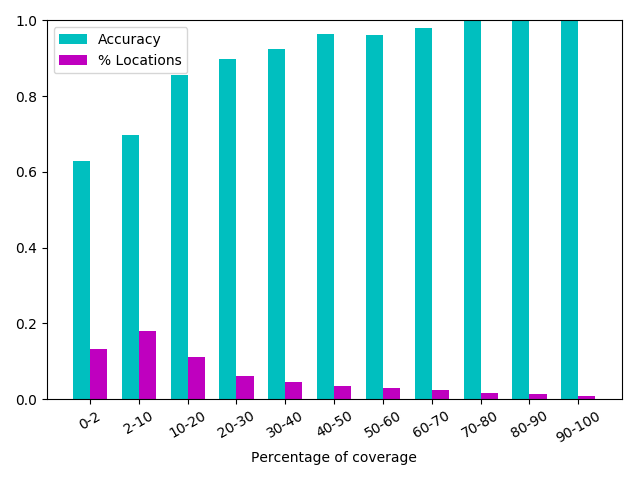
\includegraphics[width=\textwidth]{pics/d4_accuracy_vs_coverage.png}
\caption{$D_1$}
\end{minipage}
\begin{minipage}{.01\textwidth}
\end{minipage}
\begin{minipage}{.24\textwidth}
  \centering
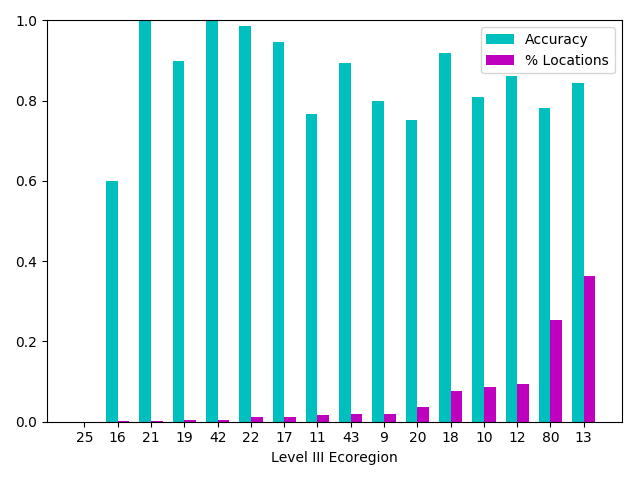
\includegraphics[width=\textwidth]{pics/d4_accuracy_vs_ecoregion.png}
\caption{$D_2$}
\end{minipage}
\begin{minipage}{.24\textwidth}
  \centering
\includegraphics[width=\textwidth]{pics/d4_accuracy_vs_landcover.png}
\caption{$D_3$}
\end{minipage}
\begin{minipage}{.01\textwidth}
\end{minipage}
\begin{minipage}{.24\textwidth}
  \centering
\includegraphics[width=\textwidth]{pics/d4_accuracy_vs_soil.png}
\caption{$D_4$}
\end{minipage}
\caption{Accuracy for different subsets of the field locations.}\label{fig:testmetrics}
\end{figure}
% accuracy versus categories
% average
\begin{figure}
\centering
\begin{minipage}{.48\textwidth}
  \centering
\includegraphics[width=\textwidth]{pics/roc.png}
\caption{ROC curves for best performing DNN models on different data subsets}
\end{minipage}
\begin{minipage}{.04\textwidth}
\end{minipage}
\begin{minipage}{.48\textwidth}
  \centering
\includegraphics[width=\textwidth]{pics/confusion_MODIS+LandSat+Niche.png}
\caption{Confusion matrix for best performing DNN model.}\label{confusion}
\end{minipage}
\end{figure}
%============================================================================================
% Subsection Performance on Full Study Region================================================
%=============================================================================================
\subsection{Performance on Full Study Region}
In this section we analyze the geographic variability in cross-validation model predictions among other things.
%\begin{figure}
%\includegraphics[width=\textwidth]{pics/modus_prob.png}
%\caption{250 meter resolution map for best deep neural network classification model.}\label{250m}
%\end{figure}
\subsubsection{Pixel-wise count of cheatgrass class across model predictions}
\subsubsection{Block statistics (count) of cheatgrass class (analogous to block area), then look at range of block counts}
%============================================================================================
%============================================================================================
%Section: Conclusion and Future Work================================================
%=============================================================================================
%============================================================================================
\section{Conclusion and Future Work}

\subsubsection*{Acknowlegements}
This work was funded by the Deep Learning for Scientific Discovery Laboratory Directed Research and Development investment at the Pacific Northwest National Laboratory. 
Pacific Northwest National Laboratory is operated for the U.S. Department of Energy by Battelle under Contract DE- AC05-76RL01830.
\nocite{*}
\bibliography{fiery}
\bibliographystyle{acm}

\end{document}
































